
> \textbf{Research status — 19 November 2026.} This chapter distinguishes implemented and reproducible software demonstrations from empirical findings requiring independent validation. Earlier numerical results and case-study interpretations are retained in the archived manuscript branch \texttt{shelf/manuscript-pre-validation-20261119}, not adopted here as validated satellite observations. The current \texttt{docs/api/v1/status/index.json} identifies the published run as \texttt{mock\_mode: true}. The manuscript must be updated again after genuine observed inputs and independent reference labels are available.

\section{Evaluation Scope and Evidence Classification}

The implementation demonstrates a reproducible workflow for structured geospatial anomaly events: provider-client interfaces, deterministic synthetic raster/time-series inputs, spectral transformations, unsupervised anomaly detection, provenance hashes, JSON/GeoJSON exports and browser-based analysis. The deployed site consists of three dashboard variants (V2, V3, V4).

For the current public demonstration, ten anomaly records are available in \texttt{docs/data/anomalies.json}, mirrored in \texttt{docs/api/v1/anomalies/index.json}. They span the following \textbf{illustrative, not empirically verified} study areas.

\begin{table}[h]
\centering
\begin{tabular}{llll}
\toprule
Demonstration area & Example analytic signal & What current public records establish & What is not established \\
\midrule
Salar de Atacama, Chile & Spectral contrasts potentially relevant to evaporation ponds & Synthetic spatial features can be processed and visualized & Actual observed pond expansion, product-level imagery provenance or independent registry matches \\
Madre de Dios, Peru & Vegetation/soil differences potentially relevant to land clearing & Synthetic samples permit testing an Isolation Forest pipeline & Actual mining/deforestation detection, linked Sentinel-1 SAR evidence or independently labeled validation pixels \\
Central Bohemia, Czechia & Night-time radiance changes potentially relevant to industrial activity & Deterministic monthly VIIRS-style series can exercise temporal detection and visualizations & Genuine observed VIIRS fluctuations or an independently reproduced correlation with regional GDP \\
\bottomrule
\end{tabular}
\end{table}
The published \texttt{docs/data/anomalies.provenance.json} lists source descriptions and hashes for mock inputs. Hash consistency is a software reproducibility property; it \textbf{does not} establish acquisition of real Sentinel imagery or corroboration by field records. The public API now records \texttt{data\_origin: synthetic\_demo} and \texttt{verification\_status: unverified} for every current anomaly.

\section{Demonstrator Functionality}

\subsection{Data Engineering}

The \texttt{pipeline.src.ingestion.SatelliteDataIngester} facade implements Earth-observation and socioeconomic provider interfaces. For the current detection run, the \texttt{fetch\_sentinel2\_data} method supplies deterministic synthetic reflectance arrays, including when a Google Earth Engine request returns a metadata-level summary. The \texttt{fetch\_viirs\_ntl} method supplies a synthetic monthly time series. This distinction prevents provider authentication or catalogue access from being mistaken for observation-level validation.

The preprocessing stage computes NDVI, NDWI and BSI over array inputs and masks unusable pixels. An Isolation Forest and temporal deviation detector produce example anomaly scores. These scores illustrate algorithmic behavior; they are \textbf{not} calibrated probabilities of a real-world event. Map coordinates and numeric sample summaries are demonstration content, not independently confirmed geospatial events.

The separate experimental GEE acquisition script, \texttt{pipeline/real\_observation.py}, has not yet demonstrated credentialed access. However, \texttt{pipeline/planetary\_observation.py} was successfully tested with a public Microsoft Planetary Computer Sentinel-2B scene on 19 November 2026: 21,253 usable observed pixels across 96×96 bounded samples in Chile (9,216), Peru (2,821) and Czechia (9,216), using five reflectance bands and SCL quality masking per source scene. The source IDs, derived-data checksums and CI proof are recorded in \texttt{docs/data/observed\_three\_region\_proof\_20261119.json}. \textbf{No independent labels, event classification or hypothesis performance were derived}, and the ten demonstration anomalies were not changed.

\subsection{Interactive Dashboards and Static API}

The public artifact provides three distinct interfaces: V2 (main spatial dashboard), V3 (science-fiction heads-up display), and V4 (institutional concept console). Satellite imagery is the default basemap on each. Dashboard interactions, map rendering, static JSON request paths and offline/PWA behavior can be tested independently of whether the underlying anomaly sample is synthetic.

The published API provides the anomaly list, individual records, dataset descriptions and a run-status snapshot. These are static JSON resources hosted by GitHub Pages; their accessibility does not mean a live sensor ingestion job is running. All three dashboards link to \texttt{docs/evidence.html}, which explains current scientific limitations.

\subsection{Software and API Verification}

At the time of the evidence review, the connected GitHub Actions repository had passing runs for strict Python lint/type checking, Python 3.12/3.13 tests, security scanning, API-health checks and GitHub Pages deployment. These verify software behavior under the tested environments. The API-health check distinguishes public endpoints returning valid data from optional authenticated providers with unconfigured credentials.

The current reproducible demonstrations and automated tests provide a technical foundation. They are \textbf{not} substitutes for ground-truth labels, documented acquisition IDs, an experimental sampling frame or external scientific review.

\section{Research Hypotheses: Current Status and Required Evidence}

\subsection{H1 — Mining and Industrial Anomaly Detection}

\textbf{Research hypothesis:} Unsupervised multivariate spectral anomaly detection can distinguish relevant extraction/clearing changes from background conditions with an F1 score greater than 0.80.

\textbf{Current status:} \textbf{Not evaluated on a verified held-out real-imagery dataset.} Earlier draft figures (including F1 = 0.907, precision = 0.936, and recall = 0.880) do not have a sufficiently traceable set of independently labeled example pixels and observed source scenes in the current public repository. They are not treated as empirical findings here.

\textbf{Required evaluation:}

\begin{enumerate}
  \item Acquire real reflectance assets with sensor/product IDs, acquisition dates, band scaling, QA/cloud masking and recorded spatial reference information.
  \item Define independent ground-truth labels with documented source rights, scene times and spatial matching protocol.
  \item Fix spatial/temporal training, tuning and held-out test splits before evaluating performance.
  \item Publish confusion matrix counts and code computing precision, recall and F1 from those exact labels.
  \item Quantify uncertainty using appropriate spatial resampling, report false positives and compare against simple baselines.

\end{enumerate}
Until all steps are completed, there is \textbf{no defensible confirmed F1 value or supported/rejected H1 decision}.

\subsection{H2 — Night-Time Lights and Economic Indicators}

\textbf{Research hypothesis:} Independently observed VIIRS DNB night-time light variations correlate with appropriately aligned macroeconomic growth observations (proposed threshold \texttt{r >= 0.65} and significance \texttt{p < 0.05}).

\textbf{Current status:} \textbf{Not evaluated on a fully evidenced pairwise time series.} Earlier draft statistics such as Pearson r = 0.724, a p-value of 0.0002 and an analysis of 21 quarters are not independently reproducible from linked real monthly VIIRS measurements and regional GDP observations in the current public artifact.

\textbf{Required evaluation:}

\begin{enumerate}
  \item Retain observed VIIRS product version, geographic footprint, calibration and quality-mask policy.
  \item Retrieve an official economic series with documented geography, definition, temporal frequency and revision vintage.
  \item Align observations by time and footprint; expose missingness instead of imputing zero economic growth.
  \item Publish the actual paired vectors and reproducible statistical calculation.
  \item Diagnose trend, seasonality, autocorrelation, sample size, multiple testing and uncertainty before interpreting statistical significance.

\end{enumerate}
Thus \textbf{H2 remains undecided}. Successful IMF/World Bank API connectivity is not, by itself, a completed correlation study.

\subsection{Spatial Autocorrelation}

Earlier draft values such as Moran's I = 0.648 and a high standardized z-score cannot be accepted as a spatial clustering result without an identified spatial weight matrix, exact observations and reproducible code. The required future analysis will specify neighborhood construction, edge effects, null distribution/permutation testing, and spatially robust evaluation splits.

\section{Performance Measurement Status}

A deterministic offline execution time is not directly comparable to downloading and preprocessing real satellite raster assets. Consequently, earlier draft values such as a 9.0-second total ETL time, 184 ingested scenes and 310 MB peak memory are \textbf{not accepted as verified production benchmarks}.

A future reproducible benchmark must record hardware, Python/dependency versions, source product counts, AOI, network conditions, image size, cloud masking, warm/cold caches, retries and at least several independent runs. Separate provider latencies from raster processing and model fitting. The current CI and tests establish functionality, not a validated real-data throughput claim.

\section{Evidence Gaps and Data Release Gate}

The next evidence release requires an observed source-asset inventory, immutable raw-data checksums, real raster processing, independently approved reference labels, holdout evaluation, error analysis and a recorded reviewer decision. Public demonstration maps must remain separated from any restricted Rota Única drone, aircraft, farm boundary or sensor assets.

For detailed implementation steps, see \texttt{THESIS\_VALIDATION\_GAPS.md}, \texttt{REAL\_OBSERVATION.md} and \texttt{docs/evidence.html} in the repository.

\textbf{Chapter conclusion:} The primary reproducible results at this stage concern the demonstrator's software architecture, transformations, API structure and deployment, not validated geographical discoveries or confirmed hypotheses.

\section{Alentejo paired-image results}
All 9,216 grid cells passed the joint mask. The archived digital-number calculation yielded 21 cells above 0.15 and its array hash was reproduced live. Applying the product offsets yielded 162 at that threshold. Both masks retained the full grid, so changing the accepted classification list did not remove cells here.\begin{center}\begin{tabular}{rr}Absolute NDVI threshold & Cells exceeding threshold \\ 0.05 & 1897 \\
0.1 & 486 \\
0.15 & 162 \\
0.2 & 61 \\\end{tabular}\end{center}\begin{figure}[ht]\centering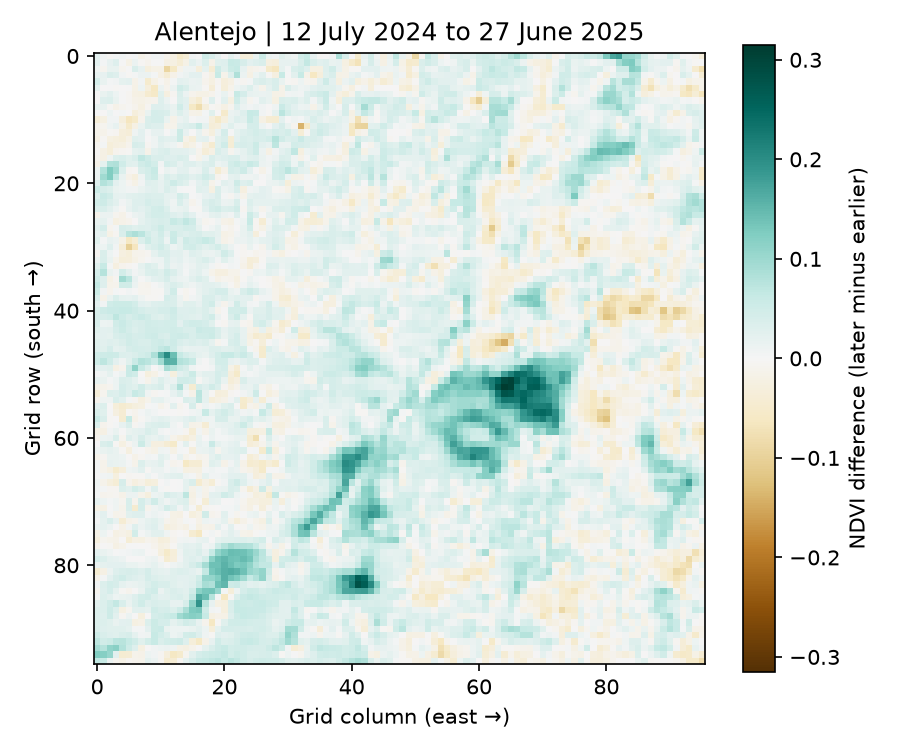
\includegraphics[width=.8\linewidth]{../../docs/data/alentejo-change.png}\caption{Paired NDVI difference on the Alentejo grid.}\end{figure}
